%************************************************
%\chapter{Background}
\chapter{Background}
\label{cap:bg}
%************************************************


Recent years have seen an increasing interest in \emph{Human Computation}
and \emph{Crowdsourcing} areas. One of the reason they are becoming
so attractive is the growth of the Web. This has allowed to leverage
on the ability of people over the Internet to perform tasks.\\

This chapter presents the main research fields related to \emph{harnessing human
intelligence to solve computational problems that are beyond the scope of existing
\ac{AI} algorithms} (\cite{human:comp}), providing a brief introduction to the
terms and the core concepts that will be used during the exposition.

Section \ref{sec:bg:crowd} gives an introduction to the concept of \emph{distributed
computing}, focusing on \emph{\ac{HC}} and \emph{Automatic computation}, from
both the theoretical point of view and to the state-of-the-art tools that
leverages on this techniques.

Section \ref{sec:bg:web} presents the web technologies that enables the 
use of the \emph{distributed computing} paradigm over the web, focusing on the
computational part of the \emph{distributed computing} process.

\section{Auto and human computation distribution}
\label{sec:bg:crowd}
%Crowd-based computation distribution

% cos'è
%% distribuzione della computazione alla massa in generale
%% comprende sia BOIC che Mturk serve per ottimizzare
%% usano infrastrutture per distribuire e recuperare i dati
% sfaccettature/specializzazioni dello stesso concetto
%% Human computation
%% GWAP
%% grid computing




Distributing computation (task computation) in the crowd means splitting
the task execution into atomic subtask that can be executed by a host (human or
not).


% nostra divisione in human e automatic
Following the subdivision presented in \autoref{tab:matrix} we subdivide the
concept of crowd-based computation distribution in two parts, \emph{Human
computation \& \ac{GWAP}} and \emph{Automatic computation}.

\subsection{Human computation \& \acs{GWAP}}
\label{sec:bg:crowd:human}
% Human computation e GWAP

\acf{HC} is a computer science technique where a computational process
performs its function by outsourcing certain steps to humans. This
\emph{outsourcing} process, as explained in the \hyperref[intro]{introduction},
is mainly due to the computational complexity of \ac{AI} algorithms. There are
some \ac{AI} problems that cannot be solved by computers or are too computational
intensive to be solved by computers in a reasonable amount of time.

Some of these are very simple tasks for humans, for example natural language
processing and object recognition are hard to solve problem for a computer,
but natural for a human being. A great example for this kind of problem
is recognizing hand-written text. Even after years of research,
humans are still faster and more accurate than computers. Other \ac{AI} problems
are too computationally expensive, such as many NP-complete problems like
Traveling Salesman problem, scheduling problems, packing problems, and FPGA
routing problems.\\

The expression \emph{\acf{HC}} in the context of computer science is already
used by \cite{cogprints499}. However is \cite{human:comp} to introduce the modern
usage of the term. It defines human computation as "\emph{a research area of
computer science that aims to build systems allowing massive collaboration between
humans and computers to solve problems that could be impossible for either to
solve alone}". A most simple and direct definition of \ac{HC} is:
\begin{quoting}\flushright
	Some problems are hard, even for the most\\
	sophisticated AI algorithms.\\
	Let humans solve it\omissis\\
	\medskip
    {\rm --- Edith Law}
\end{quoting}



\begin{figure}[htb]
    \centering
    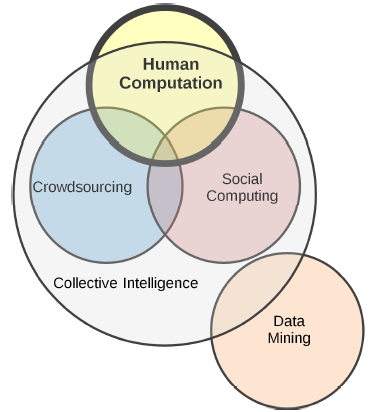
\includegraphics[width=0.6\columnwidth]{HC-relation}
    \caption{\acl{HC} relation with CrowdSourcing, Social Computing and Collective
    intelligence.}
    \label{fig:HC-relation}
\end{figure}
\acl{HC} is related with other terms, such as \emph{CrowdSourcing},
\emph{Social Computing} and \emph{Collective Intelligence} as depicted in
\autoref{fig:HC-relation}. Here we give some definitions to better understand the
similarities and the differences:
\begin{description}
    \item[CrowdSourcing] is "\emph{the act of taking a job traditionally
    performed by a designated agent (usually an employee) and outsourcing it to an
    undefined, generally large group of people in the form of an open call}"
    \cite{howe2006rise}. So it does not involve computation directly like \ac{HC}.

    \item[Social Computing] "\emph{describes any type of computing application
    in which software serves as an intermediary or a focus for a social relation}"
    \cite{schuler1994social}. So despite of the name its purpose is not computing.

    \item[Collective intelligence] defined very broadly as "\emph{groups of
    individuals doing things collectively that seem intelligent}".
\end{description}

When dealing with a human crowd the main issue is to engage users to perform tasks.
A user can be motivated to perform a task due to it's nature
(e.g. the task helps finding the cure to some disease) or to the revenue (e.g.
karma\footnote{Reputation points used in \url{www.reddit.com}.}) he/she gets for doing
such task. The most effective way for recruiting and motivating users is to give
them money\footnote{Since the ancient time. TODO ???}. For instance
\citetitle{turk} is an online tool for performing \ac{HIT} in exchange of money
rewards\footnote{The rewards for a single \ac{HIT} can be as low as 0.01\$.}.\\

\begin{figure}[htb]
    \centering
    
\includegraphics[width=\columnwidth]{HC-distribution}
    \caption{Centralized vs Distributed execution of \acl{HC}.}
    \label{fig:HC-distribution}
\end{figure}
The categorization of \ac{HC} can be further specified by adding another dimension
that involves how the tasks are executed by the users. As you can see in
\autoref{fig:HC-distribution} there are two main types of \ac{HC} execution:
\emph{centralized} and \emph{distributed}.






\subsubsection{Centralized}
In the \emph{centralized} execution we have a central hub (i.e. a website) where
users must go to perform the task. Typically the execution of a task does not
involve the offload of code and data to the user, and there is no need of ad-hoc
softwares to run the task.\\

A good example of a \emph{centralized} \ac{HC} platform is \citetitle{turk}.
\citetitle{turk} is an online platform for executing tasks in exchange of money
rewards. The platform is divided into two sections, one for the \emph{Worker}s and
one for the \emph{Requester}s. The \textbf{Worker}s are users willing to spend
time to execute a \ac{HIT} and receive the reward, the \textbf{Requester}s are
users that publish \ac{HIT} and after getting the results pay the \emph{Worker}s.\\

The lifecycle of a \ac{HIT} is the following:
\begin{enumerate}
    \item A \emph{Requester} creates a \ac{HIT} using one of the predefined project
    instances available.

    \item Once the creation is completed the \ac{HIT} is ready to be executed by
    the \emph{Worker}s.

    \item To execute a \ac{HIT} a \emph{Worker} must visit the \citetitle{turk}
    website and choose from a list of available \ac{HIT}s the one that he/she
    wants to perform (see \autoref{fig:turk}).

    \item Once the whole \ac{HIT} is completed the \emph{Requester} checks the
    result obtained and if he/she is satisfied then proceeds with the payment.
\end{enumerate}
As one can see the whole flow of the \ac{HIT} from the creation to the payment
of the \emph{Worker}s is done within the browser.\\
\begin{figure}[htb]
    \centering
    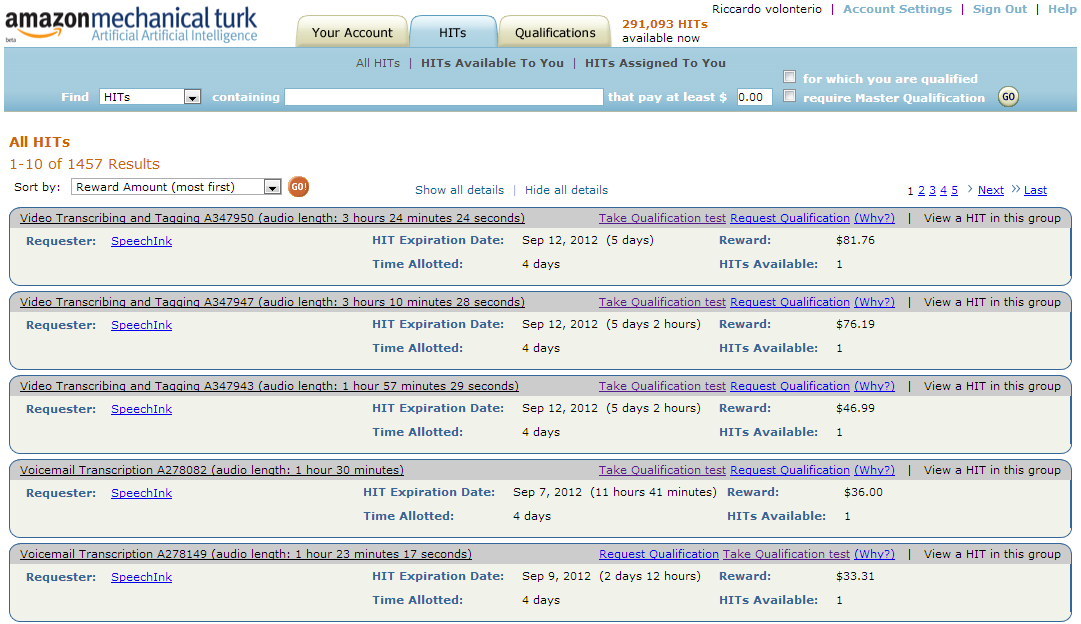
\includegraphics[width=\columnwidth]{turk}
    \caption{\citetitle{turk} web interface for choosing the \acs{HIT}.}
    \label{fig:turk}
\end{figure}


This platform has been \emph{extended} as presented in \cite{little2010turkit}
to create complete \acl{AI} algorithms able to use human computation as functions
during the execution process. The code in \autoref{lst:turkit} is an example of an
algorithm implemented using Turkit. Here \code{mturk.prompt} and \code{mturk.vote}
are \acl{HIT} executed on the \citetitle{turk} platform.
\begin{lstlisting}[language=C++,caption={Example of a Turkit algorithm.},
label={lst:turkit}]
ideas = []
for (var i = 0; i < 5; i++) {
	idea = mturk.prompt("What's fun to see in New York City? Ideas so far: " + ideas.join(", "))
	ideas.push(idea)
}
ideas.sort(function (a, b) {
	v = mturk.vote("Which is better?", [a, b])
	return v == a ? -1 : 1
})
\end{lstlisting}







\subsubsection{Distributed}
In a \emph{distributed} execution environment the central hub acts as a distribution
node in charge of offloading the task upon user request. The user can now run the
task locally without the intervention of the central hub. Eventually, when the task
is done, the user contacts the hub to upload the results.
The process of requesting the task to the hub, executing the task and sending the
results, is all done by the users, typically by a standalone piece of software
installed by the user.

% TODO ??
This solution needs the creation of ad-hoc softwares able to run on every platform
to give users an usable tool for their purpose.\\


\begin{figure}[htb]
    \centering
    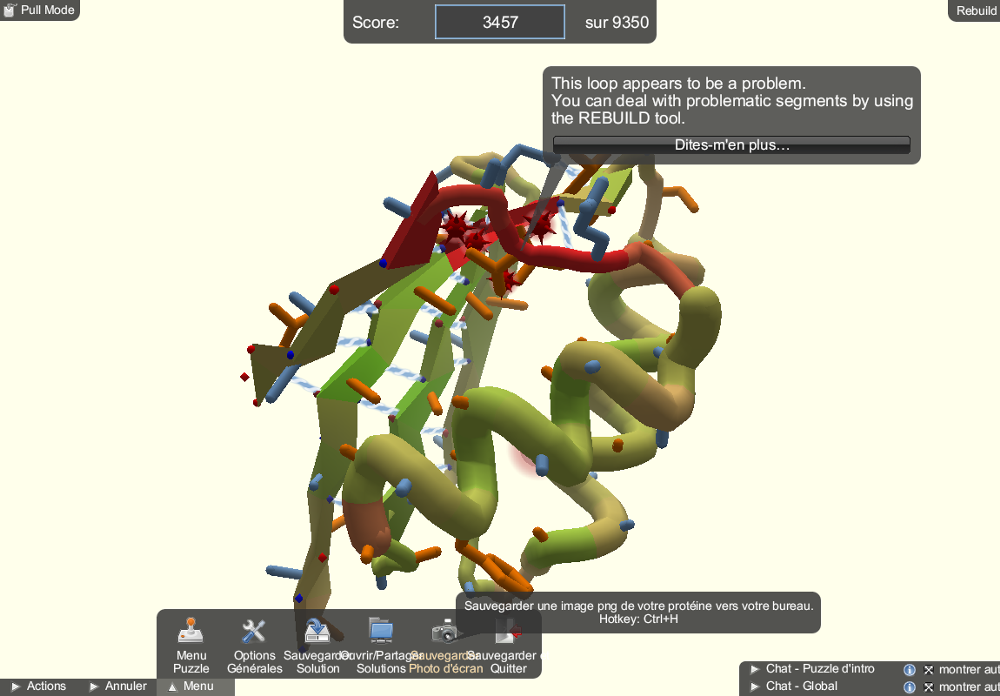
\includegraphics[width=\columnwidth]{foldit}
    \caption{The FoldIt user interface for .}
    \label{fig:foldit}
\end{figure}
An example for this kind of code distribution is the \citetitle{foldit} game.
\citetitle{foldit} is a puzzle game about protein folding, developed
by the University of Washington's Center for Game Science in collaboration with
the UW Department of Biochemistry. The objective of the game is to fold the
structure of selected proteins to the best of the player's ability. The highest
scoring solutions are analyzed by researchers, that can determine whether or not
there is a native structural configuration that can be applied to the relevant
proteins (see \autoref{fig:foldit}).







\subsubsection{\acl{GWAP}}
\acf{GWAP} is "\emph{a human-based computation technique in which a computational
process performs its function by outsourcing certain steps to humans in an
entertaining way}" von Ahn.
\ac{GWAP} come from a simple observation of data on how many hours are spent
playing games. \cite{von2008designing} reported that, accordingly to the
Entertainment Software Association\footnote{Game data from
\url{www.theesa.com/facts/gamer_data.php}}, more than 200 million hours are spent
each day playing computer and video games in the U.S.. Indeed, by age 21, the
average American has spent more than 10,000 hours playing such games equivalent
to five years of working a full-time job 40 hours per week.\\

The simple idea behind \ac{GWAP} is \emph{why not make playing games useful}?
If a task can be transformed into a game the user can be motivated to play the
game so there is no need of other types of reward (i.e. money) for doing such
task. The entertainment of playing the game itself can be used as a reward for
the user.\\

The ESP game, is a \ac{GWAP} developed by Luis von Ahn to perform image tagging.
The users' task is to agree on a word that would be an appropriate label for the
recognition of the image as described in \cite{von2004labeling}. Another \ac{GWAP}
by von Ahn is Peekaboom, where users help computers locating objects in images.

\subsection{Automatic computation}
\label{sec:bg:crowd:auto}

Unlike human computation, \emph{automatic computation} aims at executing a task, or
part of it, in an automatic fashion, without user's interaction. This kind of
\emph{distributed computation} leverages on the existence of a \emph{grid} of
connected nodes able to perform data intensive calculation.


Distributed computing deals with the execution of code on multiple computers
connected to a network. As stated in \cite{andrewsfoundations}: "\emph{Distributed
computing is a field of computer science that studies distributed systems. A
distributed system consists of multiple autonomous computers that communicate
through a computer network. The computers interact with each other in order to
achieve a common goal. A computer program that runs in a distributed system is
called a distributed program, and distributed programming is the process of
writing such programs.}"
\begin{figure}[htb]
    \centering
    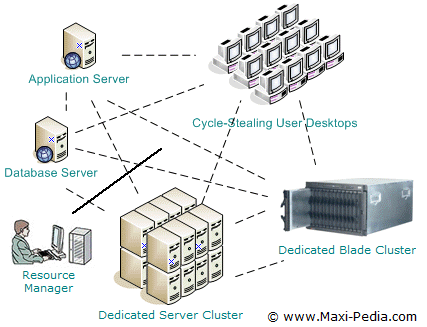
\includegraphics[width=\columnwidth]{DistributedComputing}
    \caption{General structure of a distributed computing system.}
    \label{fig:distributed-computing}
\end{figure}

% TODO ???
The platforms that implement these solution use different frameworks for splitting
algorithms into atomic operation executable by the nodes. One of these frameworks
is MapReduce\footcite{dean2008mapreduce} that, using the core concept of
\emph{Divide et impera}, can produce highly parallelizable algorithms.\\

The name "\emph{distributed computing}" refers to a wide range of different
applications (i.e. grid computing, cloud computing,
\nameref{sec:bg:crowd:auto:parasitic}, jungle computing\footnote{Winner of the
coolest name 2012}), that implement the same paradigm with different purposes.
Using the dimensions presented in \autoref{tab:matrix} we can divide the
core concept of \emph{distributed computing} into two subcategories: \emph{voluntary
computing} and \emph{parasitic computing}.


\subsubsection{Voluntary computing}
\label{sec:bg:crowd:auto:voluntary}
\emph{Voluntary computing} refers to all those \emph{distributed computation}
systems where the computation is performed on behalf of the users will. In such
systems users go to the website of the "project" they intend to support and, usually
by installing an ad-hoc client, give the resources (i.e. CPU idle time, storage,
etc.) of their machines to the chosen "project".\\

The first project implementing such computing paradigm was
\ac{GIMPS}\footnote{\url{http://www.mersenne.org/}}, started in 1995. Then other
platforms (such as \href{http://www.distributed.net/}{distributed.net},
\href{http://setiathome.berkeley.edu/}{SETI@home}, etc. ) have been developed to
support this type of computation.

\begin{figure}[htb]
    \centering
    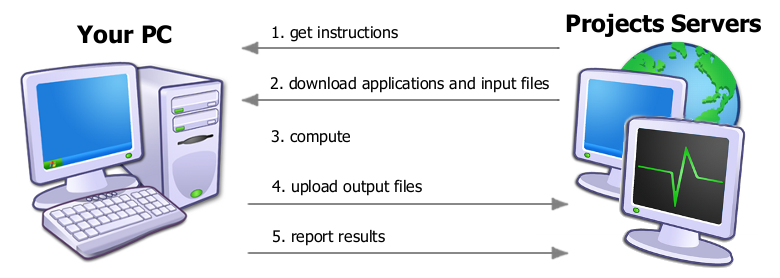
\includegraphics[width=0.8\columnwidth]{boinc}
    \caption{The \acs{BOINC} computational flow.}
    \label{fig:boinc}
\end{figure}
\acf{BOINC}\footnote{\url{http://boinc.berkeley.edu/}} is an open-source software
for Voluntary computing and grid computing. \ac{BOINC} was originally developed
to support the \acf{SETI@home} project, before it became used as a platform for
other distributed computing applications. It consists of two parts: the back-end
server, running on Linux platforms, and the client, cross-platform, for the
end-user computing.\\

The client software allows users to connect to the \ac{BOINC} grid, to perform
computation. The flow of the execution, as depicted in \autoref{fig:boinc} is
the standard \emph{distributed computing}. Here is the list of actions performed
to run the task on the client:
\begin{enumerate}
    \item get instruction from the server on how to get all the resources needed
    to perform the task
    \item download all the resources from the server
    \item execute the downloaded application
    \item send the results obtained to the server
\end{enumerate}

There are over 40, at the time of writing, projects that leverage on
the \ac{BOINC} platform to perform computation on different application areas.
For example the aforementioned \ac{SETI@home} project uses this framework to
search for extraterrestrial intelligence by analyzing the narrow-band radio
signal coming from the Arecibo radio telescope.


\subsubsection{Parasitic computing}
\label{sec:bg:crowd:auto:parasitic}
% Spiego l'idea
% chi è stato
% e perchè
% come funziona

Parasitic computing\footnote{In this thesis we are not covering, neither
we are interested in, the ethical or moral implication of using this technique.}
is a technique that, using some exploits and ad-hoc code, allow a \emph{malicious}
user to use the computational power of the \emph{victim} computer without this
being aware. As one can notice parassitic compiting has a strong relationship
with \emph{distributed computing}, in fact is a specialization of the general
class of \emph{voluntary computing}, where the user is unaware of
the execution\footnote{In \emph{voluntary computing} the user can be unaware
of the actual code they are executing, but they are aware of the execution.}.\\

This approach was first proposed by \cite{barabasi2001parasitic} to solve the
NP-complete 3-SAT problem using the existing TCP/IP protocol stack and its error
handling routines. The satisfiability problems or "SAT" involves finding a
solution to a boolean equation that satisfies a number of logical clauses. For
example, $(x_1 \oplus x_2) \land (x_2 \land x_3 )$ in principle has $2^3$ potential
solutions, but it is satisfied only by the solution: $x_1=1, x_2=0, x_3=1$.
Problems problem like the one in the example are known as 2-SAT problem because
each clause, shown in parentheses, involves two variables. The more difficult
3-SAT problem is known to be NP-complete, which in practice means that there is
no known polynomial-time algorithm which solves it.\\
\begin{figure}[htb]
    \centering
    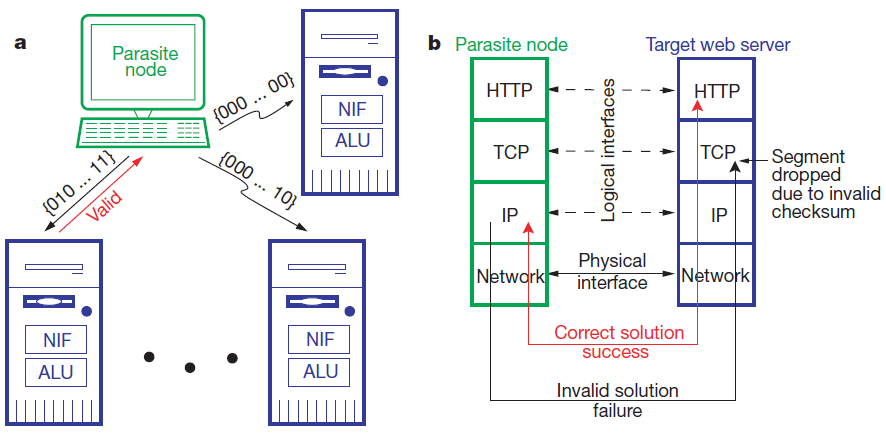
\includegraphics[width=\columnwidth]{parasitic}
    \caption{Schematic diagram of the parasitic computer solving the 3-SAT
    problem.}
    \label{fig:parasitic}
\end{figure}

The approach proposed in the paper was to perform a brute force attack to guess
the right solution of a 3-SAT problem using a parallel apprach as depicted in
\autoref{fig:parasitic}. The parasite node creates $2^n$ specially constructed
messages designed to evaluate a potential solution. These messages are sent to
many target servers throughout the Internet. After receiving the message, the
target server verifies the data integrity of the TCP segment by calculating a
TCP checksum. The construction of the message ensures that the TCP checksum fails
for all messages containing an invalid solution to the posed SAT problem. Thus,
a message that passes the TCP checksum contains a correct solution. The target
server will respond to each message it receives (even if it does not understand
the request). As a result, all messages containing invalid solutions are dropped
in the TCP layer. Only a message which encodes a valid solution \emph{reaches}
the target server, which sends a response to the \emph{request} it received.\\

This approach may seem wrong or at leat not right, with respect to the user, but
if one think about it notice how we are always making computation without even
knowing. \ac{GWAP} or application like \href{http://www.google.com/recaptcha}{reCAPTCHA}
are examples of involuntary human computation (as in \autoref{tab:matrix}). So
they are using the same technique to perform a sort of \emph{parasitic human
computing} without complainig about the user will.\\

To avoid the ethic implication of doing \emph{parasitic computing} a hybrid
approach (parasitic/voluntary) can be used. If the user give the permission to
run computation on its computer exchange of a return of any type, then we are
able to score the best on both approaches. A similar solution was proposed in
\cite{karame2011pay}.
In this paper they propose a microcomputations as micropayments in web-based
services. Their solution is to give the user access to online contents (such as
newspaper, video, etc.) after performing small \js{} computation.

\paragraph{Parasitic \js{}} described in \cite{jenkin2008parasitic} can be
considered an enhancement of the solution proposed by \cite{barabasi2001parasitic},
since using \js{} and the HTML5 features to their full potential (see
\ref{sec:bg:web:html5}) we are able to perform any kind of computation
within the browser window/tab. \js{} offers also a standard platform for the
exection of code without the need of any ad-hoc software for each platform.
Furthermore all the code executed by a browser run in a sandboxed environment,
keeping the user computer safe from any malicuis intent.



\section{Enabling web-based distributed computation}
\label{sec:bg:web}
% Enabling web-based distributed computation

Using the web (i.e. the browser) as a platform for distributing and executing
code implies that we have the available technologies to perform high-level
\emph{computation} and real-time \emph{communication}. These are the requirements
for evaluating the web as a suitable platform for code distribution.\\

\paragraph{Computation} is the key for being able to perform tasks within the
browser. \emph{Computation} can involve any kind of operation on the data, and
the data itself can be of any type. For instance creating an application that
analyzes audio files, or creating a image manipulation program that runs without
external plugins is relatively simple using standard languages (e.g. C, C++,
Java, etc). Until a few years ago it was almost\footnote{Without using strange
interaction between Flash/Silverlight and the browser.} impossible to do it within
a browser.

HTML5 filled the gap that existed between any "standard" language and \js{}
giving the developers access to all the required APIs needed to create fully
functional web-applications. In \ref{sec:bg:web:html5} are presented all the
features, along with some technical details, that have enabled this evolution.\\

There are also initiatives that aim at simplify the deployment of \js{}
application. Since most of the developers have experience on languages other than
\js{} there is the need of porting existing application to the Web.
Projects like \citetitle{emscripten} and \citetitle{gwt}
offer the possibility to write the code directly in C,C++ (\citetitle{emscripten})
or Java (\citetitle{gwt}) and compile it into pure, and optimized, \js{}.

\citetitle{emscripten}, by Mozilla, is a LLVM-to-JavaScript compiler. It takes
LLVM bitcode (which can be generated from C/C++ using Clang, or any other
language that can be converted into LLVM bitcode) and compiles that into \js{}.
Since it is a compiler it offers multiple grades of optimization that reduce the
size of the \js{} file and speedup the computation. The website is full of demos
of the ported application, including games, 2D/3D game engines, various libraries
and also SQLite.

\citetitle{gwt}, by Google, is a development toolkit for building and optimizing
complex browser-based applications. Its goal is to enable productive development
of high-performance web applications without the developer having to be an expert
in browser quirks, XMLHttpRequest, and \js{}.\\



\paragraph{Communication} is being empowered by
introducing \emph{WebSocket}, that enables full-duplex data exchange with the
server, and \ac{CORS} that gives the developers the possibility to make \ac{AJAX}
requests to "foreign" servers (other than \code{localhost}) without the need of
a proxy for forwarding the requests.\\


% TODO non mi convince
The availability of all those technical API gives the possibility to create a
system capable of performing any \emph{Human} or \emph{Automatic} computation
task without the need of external plugins. We used all the features of HTML5
for the computation side of the System. WebSocket are used for real-time task
monitoring and \ac{CORS} are used within the task to request any
external data needed by the application.

\subsection{\acs{HTML}5}
\label{sec:bg:web:html5}
\begin{figure}[htb]
    \centering
    
\includegraphics[width=0.75\columnwidth]{HTML5logos}
    \caption{Official HTML5 logo \& unofficial CSS3 logo.}
    \label{fig:html-logos}
\end{figure}

When speaking of \ac{HTML}5 one, usually, is not only focusing on the markup language
but on a set of web technologies and specifications strictly related to \ac{HTML}5.
This set of technologies includes the \ac{HTML}5 specification itself, the
\ac{CSS}3 recommendations and a whole new set of \js{} APIs. So, first things
first, let us point out the differences:
\begin{description}
	\item[HTML5] refers to a set of semantic tags (like \ctag{footer},
	\ctag{header}, \ctag{article}, \ldots), media tags (like \ctag{video} or
	\ctag{audio}) and the so called Web Form 2.0 alongside with all the "old"
	tags inherited from HTML4. These tags help developers to give semantics to
	the website they make, so the websites can be
	better understood by search engines or HTML parsers (like those used for
	reading the site for blind people).

	\item[CSS3] refers to the presentation layer of the pages. Here are introduced
	specifications including image effects, 3D transformation, new tag selectors, 
	form element validation, etc. The specifications take care also of the new
	devices (like smartphones and tablets) giving the user the \code{media
	queries} to examine the media (screen, print, aural) and provide different
	\ac{CSS} rules.
	
	\item[JS] refers to the \js{} with a new set of API for interacting with the
	new media elements and other tags, as long as API for concurrent computation,
	real-time communication, offline storage, etc.\\
\end{description}

With the advent of \ac{HTML}5, like any new technology, many problems were
resolved and many others have been created. The main issue with using \ac{HTML}5
is the browser compatibility and browser-specific methods.

When browsers start
implementing some \ac{HTML}5 draft feature, since they are not fully standardized
\footnote{In fact HTML5 (at the time of writing) is not yet standardized, its
still a draft. See \url{http://www.w3.org/TR/html5/}}, they prevent the pollution
of the DOM by prefixing the standard method
with a browser specific prefix\footnote{\code{o}: for
Opera, \code{ms}: for Internet Explorer, \code{moz}: for Firefox, and
\code{webkit}: for the WebKit based browser (Chrome and Safari)}(i.e.
\linebreak\code{requestAnimFrame}
can become \code{mozRequestAnimFrame} or \code{webkitRequestAnimFrame}). This prefixing
is particularly common in the \ac{CSS}3 where things becomes awful\footnote{See
CSS animation or gradients for example.}.\\


To avoid browser inconsistency there are plenty of \js{} frameworks for every
purpose. Frameworks like \citetitle{jquery} provide a layer of abstraction between
browser-specific code and the user, giving developers fallbacks for the most
common API and additional features not covered by the standard implementation.
Other frameworks like \citetitle{modernizr} give developers the ability to test
if some \ac{HTML}5 feature is available in the currently used browser and provide
a general fallback system for dynamically load polyfills\footnote{A polyfill is
a \js{} library or third part plugin that emulates one or more HTML5 feature,
providing websites to have a consistent behavior.}.\\


Now are presented the main \ac{HTML}5 features to better understand how they can
be used in this System.





\paragraph{Canvas}
Let's start with the official definition\footnote{Got from the specs:
\url{http://www.w3.org/TR/html5/the-canvas-element.html\#the-canvas-element}}
\begin{quoting}\rm\tt
	The canvas element provides scripts with a resolution-dependent bitmap canvas, which can
	be used for rendering graphs, game graphics, or other visual images on the fly.
\end{quoting}

So the \code{canvas} element is basically a \emph{Canvas}, like the name says, where
one can \emph{paint} anything. On top of this, the \code{canvas} element gives
the developers access to the underlying raw pixel data. Also in the \code{canvas}
element you can \emph{draw} images taken from a \ctag{img} tag or a frame taken
from a \ctag{video} tag.

As one can see now we have all the tools we need to perform image analysis or
video manipulation within the browser. Obviously there are plenty of \js{}
libraries that facilitate the whole process of filtering or, in general, image
manipulation (like \href{http://www.pixastic.com/}{Pixastic} or
\href{http://camanjs.com/}{Camanjs}). Other libraries give you the tools to
create diagrams or charts on the fly (like \href{http://raphaeljs.com/}{Raphaël}
or \href{http://processingjs.org/}{Processingjs}).

The canvas element also provides a 3D context to draw and animate
\footnote{Animations are not natively supported, must be coded separately.}
high definition graphics and models using the WebGL API. This API is maintained
by the \href{http://www.khronos.org/}{Khronos Group} and is based on OpenGL ES
2.0 specifications. On top of these API there are a lot of libraries\footnote{For
a reference see \url{http://en.wikipedia.org/wiki/WebGL\#Developer_libraries}}
made to facilitate development of 3D applications. One of the the most used is
the \href{http://mrdoob.github.com/three.js/}{Three} \js{} library, that can be
used for creating and animating 2D or 3D scenes within the canvas element.








\paragraph{WebSocket}
The WebSocket is an API interface for enabling bi-directional full-duplex client
server communication on top of the \ac{TCP}. It enables real-time
communication between clients and servers, allowing servers to \textbf{push} data
to the clients and obtain \emph{real} real-time content updates.

Like many other \ac{HTML}5 features on top of WebSocket a library that
provides easy access to these functionality as long as fallbacks for old browsers
was built.
\citetitle{socket.io} provides a single entry-point to create a connection to the
server and manage the message exchange, providing fallbacks\footnote{If WebSocket,
are not available the library can use Adobe\reg Flash\reg Socket, AJAX long
polling, AJAX multi-part streaming, Forever Iframe and JSONP Polling} to ensure
cross-browser compatibility.





\paragraph{WebWorkers}\label{html5:workers}
A problem that rises when coding load intensive \js{} application is the single thread nature
of the language. Every script runs in the same thread of the browser window/tab.
This can lead to some unwanted behavior (like browser freezing or a warning
dialog that that alerts the user as in \autoref{fig:browser-slow-dialog}).
\begin{figure}[htb]
    \centering
    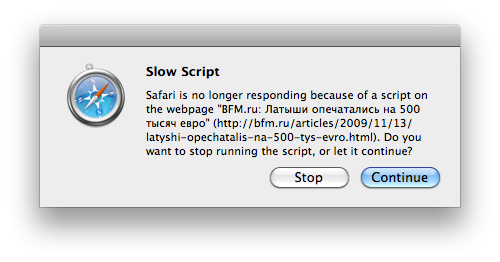
\includegraphics[width=0.75\columnwidth]{browser-slow-dialog}
    \caption{The slow script dialog.}
    \label{fig:browser-slow-dialog}
\end{figure}
To solve this problem \cite{jenkin2008parasitic} proposed a timed-based
programming structure that ensures that the code runs without any browser warning
or freezing and also offers the developer to tweak the performance of the script
by dynamically adjusting the interval between the step execution. This method
leverage on the \code{setTimeout} function of \js{} in order to split code into
timestep-driven code chunks to execute. Here is an example of loop translated
into a timer-based loop:
\begin{multicols}{2}
	\begin{algorithm}[H]
		\While{condition}{
			...do something...
		}
	\end{algorithm}

	\vfill
	\columnbreak

	\begin{algorithm}[H]
		\SetKwBlock{procedure}{procedure}{}
		\SetKwFunction{setTimeout}{setTimeout}

		\procedure(STEP){
			...do something...\\
			\If{condition}{
				\setTimeout{STEP, delay}
			}
		}
	\end{algorithm}
\end{multicols}
Obviously this is not the solution to the problem, it is a hack that tricks the
browser.\\


WebWorkers offer a simpler solution. They provide a simple, yet powerful, way of
creating \emph{threads} in \js{}. The official definition says:
\begin{quoting}\rm\tt
	The WebWorkers specification defines an API for running scripts in the
	background independently of any user interface scripts.	This allows for
	long-running scripts that are not interrupted by scripts that respond to
	clicks or other user interactions, and allows long tasks to be executed
	without yielding to keep the page responsive.
\end{quoting}

The core concept behind WebWorkers is the \code{Worker}. A \code{Worker} is a
piece of \js{} code that runs in parallel to the main thread and is able to send
and receive messages (just like normal threads).



\paragraph{Storage}
When web developers think of storing anything about the user, they immediately
think of uploading to the server. \ac{HTML}5 changes that, as there are now
several technologies allowing the \ac{RIA} to save data on the client device.

\ac{HTML}5 supports a number of storage techniques able to store data within the
browser to be accessed later. Here is a simple list with the principal features:
\begin{description}
	\item[Web storage] is a convenient form for offline storage. It uses a simple
	key-value mapping for storing data persistently on the browser.

	\item[Web SQL database] is an offline SQL database, usually implemented using
	SQLite, a general-purpose open-source SQL engine.

	\item[IndexedDB] is a nice compromise between Web Storage and Web SQL Database.
	Like the former, it is relatively simple and like the latter, it's capable
	of being very fast. It uses the same mapping as \emph{Web storage} and indexes
	certain fields inside the stored data.

	\item[Filesystem API], as the name says, offers the ability to manipulate the
	file system of the host.
\end{description}


\paragraph{Offline storage}
In this category falls the \code{application cache}. The \code{application cache} is
controlled by a plain text file called a \code{manifest}, which contains a list
of resources to be stored for use when there is no network connectivity. The list
can also define the conditions for caching, such as which pages should never be
cached and even what to show the user when he follows a link to an uncached page.

If the user goes offline but has visited the site while online, the cached
resources will be loaded so the user can still view the site in a limited form.
Here is a simple cache file:
\begin{lstlisting}[language=make]
CACHE MANIFEST
      
# This is a comment

CACHE:
/css/screen.css
/css/offline.css
/js/screen.js
/img/logo.png

http://example.com/css/styles.css

FALLBACK:
/ /offline.html

NETWORK:
*
\end{lstlisting}


\subsection{WebCL}
\label{sec:bg:web:webcl}
With the advent of \ac{GPGPU}, the spreading of multicore CPUs and multiprocessor programming (like OpenMP)
we can see emerging an intersection in parallel computing. This intersection is known as
\textbf{heterogeneus computing}. \ac{OpenCL} is a framework for heterogeneus compute resources and so
\ac{WebCL} is a porting of this technlogy to the web.
% Spiego meglio perchè è nato?

\ac{OpenCL} uses a language based on C99\footnote{A programming language dialect for the past C developed in
1999 (formal name ISO/IEC 9899:1999)} for writing \emph{kernels}, functions that actually execute on OpenCL
devices. 
% come funziona OpenCL

% Problema delle prestazioni - FATTO
The main focus when building high-end web-application like 3D games is responsiveness. Altough \js{}
can be optimized and parallelized (see \vref{sec:bg:web:html5}) it cannot be fast as an application
software, because \js{} must be interpreted by the browser and then executed as machine code. \ac{WebCL}
provide an easy framework for building and running machine code in parallel directly from the browser.

% Implementazioni
%% common API 
% prestazioni, esempi
% integrazione con webGL
